\documentclass[pdf,aspectratio=169]{beamer}
\usepackage[]{hyperref,graphicx,siunitx,booktabs,lmodern}
\usepackage{physics}
\usepackage{em-commands}
\mode<presentation>{\usetheme{EM}}

%Question Numbering
\newcounter{questionnumber}
\newcommand{\qnum}{%
	\stepcounter{questionnumber}%
	Q\arabic{questionnumber}
}
\resetcounteronoverlays{questionnumber}

\graphicspath{ {../Images/} }

\sisetup{per-mode=symbol}

\tikzstyle{plate}=[draw, very thick, minimum width=4cm, minimum height=1cm, fill=gray!40, anchor=south]

%preamble
\title{Nature and Faraday Abhor Change}
\date{December 3, 2018}
\author{Jed Rembold}

\begin{document}
\renewcommand{\theenumi}{\Alph{enumi}}

\begin{frame}{Announcements}
	\begin{itemize}
		\item Homework
			\begin{itemize}
				\item Homework 12 due Wednesday night!
				\item I'm all caught up on other homework grading
			\end{itemize}
		\item Grade reports posted!
		\item Final
			\begin{itemize}
				\item Coming at you Friday!
				\item Due the 14th at 5pm
				\item Probably looking at around 5-6 problems
				\item Chapters 6 and 7 will be weighted a bit heavier, but it is comprehensive
				\item Come the moment I send it out, my solutions sets will be locked down (figuratively)
				\item Computation mainly plotting, Sympy for math help, and relaxation method
			\end{itemize}
		\item Read through 7.3.3 for Wednesday
	\end{itemize}
\end{frame}

\begin{frame}{\qnum}
	A rectangular metal loop moves through the region of constant uniform magnetic field $\mf$ with speed $v$ at a particular time. What is the magnetic force on the \emph{loop} at this instant? You can assume the loop has some overall resistance $R$.
	\begin{columns}
		\column{0.5\textwidth}
		\begin{center}
			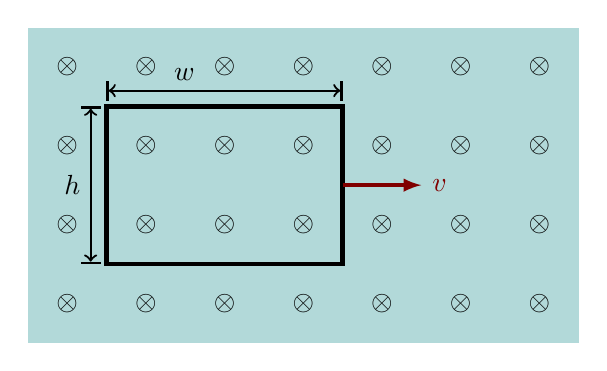
\begin{tikzpicture}
				\fill[Teal!30] (-.5,-.5) rectangle (6.5,3.5);
				\foreach \x in {0,1,...,6}{
					\foreach \y in {0,1,...,3}{
						\node at (\x,\y) {$\otimes$};
					}
				}
				\draw[ultra thick] (.5,.5) rectangle +(3,2);
				\draw[very thick, -latex, red!50!black] (3.5,1.5) -- +(1,0) node[right] {$v$};
				\path[|<->|,thick]
					(.3,.5) edge node[midway,left] {$h$} +(0,2)
					(.5,2.7) edge node[pos=.33,above] {$w$} +(3,0);
			\end{tikzpicture}
		\end{center}
		\column{0.5\textwidth}
		\begin{enumerate}
			\item \alert<2>{0}
			\item $\displaystyle \frac{vB^2 h^2}{R}$ to the left
			\item $\displaystyle \frac{2vB^2 h^2}{R}$ to the left
			\item $\displaystyle \frac{2vB^2 h^2}{R}$ to the right
		\end{enumerate}
	\end{columns}
\end{frame}

\begin{frame}{\qnum}
	A stationary rectangular metal loop is in a region of uniform $\mf$ which has a magnitude which is decreasing with time:
	\[B = B_0 - kt\]
	What is the direction of the magentic field generated by the induced current in the loop? (Say at the center of the loop.)
	\begin{columns}
		\column{0.3\textwidth}
		\begin{enumerate}
			\item \alert<2>{Into the page}
			\item Out of the page
			\item To the left
			\item To the right
		\end{enumerate}
		\column{0.7\textwidth}
		\begin{center}
			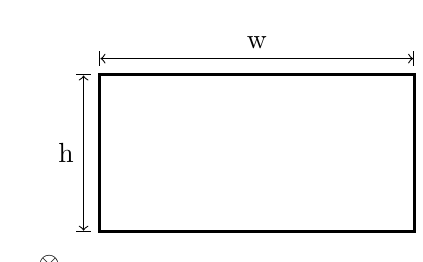
\begin{tikzpicture}
				\unifield{6}{3}{$\otimes$}{Teal!30!white}
				\draw[very thick] (.5,.5) rectangle +(4,2);
				\path[|<->|]
					(.3,.5) edge node[midway,left]{h} +(0,2)
					(.5,2.7) edge node[midway,above]{w} +(4,0);
			\end{tikzpicture}
		\end{center}
	\end{columns}
\end{frame}

\begin{frame}{\qnum}
	\begin{columns}
		\column{0.5\textwidth}
		A loop of wire is near a long straight wire which is carrying a large current $\mcur$ which happens to be decreasing. The loop and the straight wire are the same plane and are positioned as shown. The current induced in the loop is:
		\begin{enumerate}
			\item CCW
			\item \alert<2>{CW}
			\item 0
			\item Not enough info to say
		\end{enumerate}
		
		\column{0.5\textwidth}
		\begin{center}
			\begin{tikzpicture}
				\draw[very thick, Red, ->>-=.1 to 1 by .2] (0,0) -- +(5,0) node[right] {$\mcur$};
				\draw[ultra thick] (2.5,-2) circle (1);
			\end{tikzpicture}
		\end{center}
	\end{columns}
\end{frame}

\begin{frame}{\qnum}
	\begin{columns}
		\column{0.5\textwidth}
		The current in an infinite solenoid with uniform magnetic field is increasing such that $B = B_0 + kt$. A small circular loop of radius $r$ is placed off-center inside the solenoid.

		What is the emf around the small loop?
		\begin{enumerate}
			\item \alert<2>{$k\pi r^2$}
			\item $-k\pi r^2$
			\item 0
			\item Non-zero but need more info
		\end{enumerate}
		
		\column{0.5\textwidth}
		\begin{center}
			\begin{tikzpicture}
				\node[font=\Large,above] at (0,3) {Top View};
				\draw[very thick, fill=Red!70] (0,0) circle (3);
				\draw[very thick, ->>-=.1 to .9 by .2] (0,0) arc (0:-360:1);
				\draw[<->] (0,0) -- (-1,0) node[above,math, midway] {r};
				\node[label=B] at (2,0) {$\odot$};
			\end{tikzpicture}
		\end{center}
	\end{columns}
\end{frame}

\begin{frame}{\qnum}
	\begin{columns}
		\column{0.5\textwidth}
		\begin{center}
			\begin{tikzpicture}
				\node[font=\Large,above] at (0,2) {Top View};
				\draw[very thick, fill=Red!70] (0,0) circle (2);
				\draw[very thick, ->>-=.1 to .9 by .2] (-2.5,0) arc (0:-360:1);
				\draw[<->] (-2.5,0) -- +(-1,0) node[above,math, midway] {r};
				\node[label=B] at (0,0) {$\odot$};
			\end{tikzpicture}
		\end{center}

		\column{0.5\textwidth}
		The current in an infinite solenoid with uniform magnetic field is increasing such that $B = B_0 + kt$. A small circular loop of radius $r$ is placed outside the solenoid..

		What is the emf around the small loop?
		\begin{enumerate}
			\item $k\pi r^2$
			\item $-k\pi r^2$
			\item \alert<2>{0}
			\item Non-zero but need more info
		\end{enumerate}
	\end{columns}
\end{frame}

\begin{frame}{\qnum}
	\begin{columns}
		\column{0.5\textwidth}
		The current in an infinite solenoid with uniform magnetic field is increasing such that $B = B_0 + kt$. If you calculate the potential between points A and B along two different paths, do you get the same answer?

		\begin{enumerate}
			\item Yes
			\item \alert<2>{No}
			\item Can't tell with current info
			\item Only at certain times
		\end{enumerate}
		
		\column{0.5\textwidth}
		\begin{center}
			\begin{tikzpicture}[use quick Hobby shortcut]
				\node[font=\Large,above] at (0,3) {Top View};
				\draw[very thick, fill=Red!70] (0,0) circle (2);
				\node[label=$\mf$] at (0,0) {$\odot$};
				\node[point,label=A](A) at (45:2.5) {};
				\node[point,label={200:B}](B) at (180+45:2.5) {};

				\draw[very thick, ->>-=0.1 to .9 by .2] (A) to[quick curve through={(90:2.5) (135:3) (180:2.25)}] (B);
				\draw[very thick, ->>-=0.1 to .9 by .2] (A) to[quick curve through={(0:3) (-45:2.25) (-90:2.5)}] (B);
			\end{tikzpicture}
		\end{center}
	\end{columns}
\end{frame}




\end{document}
